\section{A reproducibility crisis}
\begin{frame}
\centering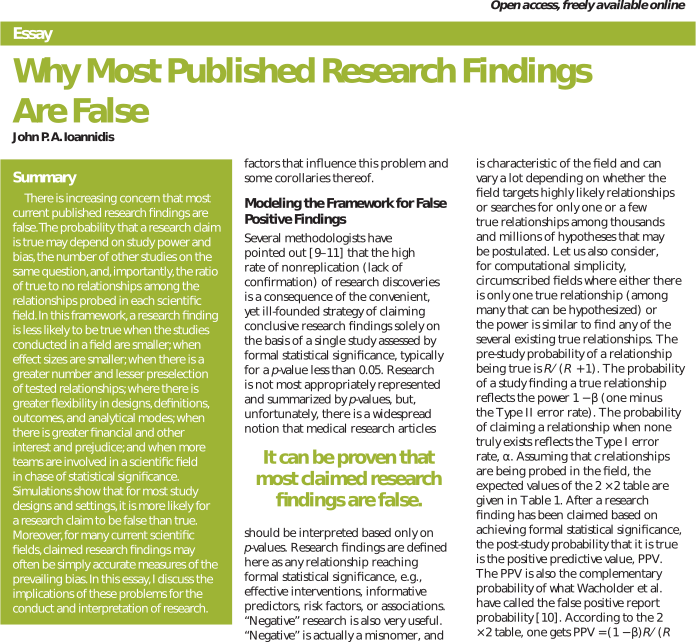
\includegraphics[scale=0.4]{images/reproduce_crisis_paper.pdf}
\end{frame}

\begin{frame}
\begin{block}{Crisis elements}
\begin{itemize}
\item Highlighted around 2005
\item Since 2010 more articles related to the non reproducibility
\item Medecine is one of the most impacted discipline
\end{itemize}
\end{block}
\end{frame}

\begin{frame}
\includegraphics[page=4,scale=0.55]{01_OS_and_FAIR_intro.pdf}
\end{frame}

\begin{frame}
\includegraphics[page=5,scale=0.55]{01_OS_and_FAIR_intro.pdf}
\end{frame}

\begin{frame}
\includegraphics[page=6,scale=0.55]{01_OS_and_FAIR_intro.pdf}
\end{frame}

\begin{frame}
\includegraphics[page=7,scale=0.55]{01_OS_and_FAIR_intro.pdf}
\end{frame}


\section{Open science and FAIR}
\begin{frame}
\begin{block}{FAIR history}
\begin{itemize}
\item Born in 2016 with \textit{The FAIR Guiding Principles for scientific data management and stewardship}
\item How to build, stock, share, use and publish data
\item Make criteria to better use our data
\end{itemize}
\end{block}
\blfootnote{\url{https://doi.org/10.1038/sdata.2016.18}}
\end{frame}

\begin{frame}
\centering
\includegraphics[scale=0.6]{images/fair_paper_2016_crop.pdf}
\end{frame}

\begin{frame}
\includegraphics[page=8,scale=0.55]{01_OS_and_FAIR_intro.pdf}
\end{frame}

\begin{frame}
\begin{block}{Findable}
\begin{itemize}
\item Easy to find
\item Unique ID
\item Rich and indexed metadata
\end{itemize}
\end{block}
\end{frame}

\begin{frame}
\includegraphics[page=9,scale=0.55]{01_OS_and_FAIR_intro.pdf}
\end{frame}

\begin{frame}
\begin{block}{Accessible}
\begin{itemize}
\item Not only open
\item But accessible with a standard protocol
\item Known licence use
\item Available metadata
\end{itemize}
\end{block}
\end{frame}

\begin{frame}
\includegraphics[page=10,scale=0.55]{01_OS_and_FAIR_intro.pdf}
\end{frame}
\begin{frame}
\begin{block}{Interoperable}
\begin{itemize}
\item Standardized metadata
\item Standardized data
\end{itemize}
\end{block}
\end{frame}

\begin{frame}
\includegraphics[page=11,scale=0.55]{01_OS_and_FAIR_intro.pdf}
\end{frame}

\begin{frame}
\includegraphics[page=12,scale=0.6]{01_OS_and_FAIR_intro.pdf}
\end{frame}

\begin{frame}
\includegraphics[page=13,scale=0.6]{01_OS_and_FAIR_intro.pdf}
\end{frame}


\begin{frame}{FAIR session with AuBi}
%\begin{block}{\textbf{F}easibility\textbf{A}ccessibility\textbf{I}nteroperability\textbf{R}eproducibility}
%\begin{itemize}
%\item Render a reproducible work in bioinformatic
%\item Introduction to the FAIR concepts
%\item FAIR training since 2019
%\item Publication related \url{https://jose.theoj.org/papers/10.21105/jose.00068}
%\end{itemize}
%\end{block}

\begin{block}{Objectives}<1->
\begin{itemize}
\item Discover FAIR practices
\item Discover tools for best practices
\item Use tool and best practices in practice sessions
\item 5 sessions for courses and practices
	\begin{itemize}
	\item Day 1: Introduction to FAIR training and Git
	\item Day 2: Git practice
	\item Day 3: Encapsulation course
	\item Day 4: Encapsulation training
	\item Day 5: Documentation course and training
	\end{itemize}
\end{itemize}
\end{block}
\end{frame}
\section{Training content}
\begin{frame}
\begin{block}{Contents}
\begin{itemize}
\item<1-> Introduction to FAIR practices
\item<2-> Code control using Git \faGit* 
	\begin{itemize}[<2->]
	\item Git environment
	\item Gitlab and Github \faGithub \faGitlab
	\end{itemize}
\item<3-> Encapsulation process
	\begin{itemize}[<3->]
	\item Conda environment and packages use \includegraphics[scale=0.07]{images/conda_logo.pdf}
	\item Containers as docker \& singularity \faDocker 
	\item Reproducible workflow using snakemake 	\includegraphics[scale=0.05]{images/snakemake_logo.png}
	\end{itemize}
\item<4-> Literate programming and documentation
	\begin{itemize}[<4->]
	\item Markdown syntax \faMarkdown
	\item Rmarkdown for R \faRProject 
	\item Jupyterlab for Python \faPython
	\end{itemize}
\end{itemize}
\end{block}
\end{frame}

